\documentclass[preprint]{sigplanconf}

\usepackage{stmaryrd}
\usepackage{epsfig}
\usepackage{alltt}
\usepackage{times}
\usepackage{code}

\newcommand{\cut}[1]{}

\newcommand{\appref}[1]{Appendix~\ref{#1}}
\newcommand{\secref}[1]{Section~\ref{#1}}
\newcommand{\tblref}[1]{Table~\ref{#1}}
\newcommand{\figref}[1]{Figure~\ref{#1}}
\newcommand{\listingref}[1]{Listing~\ref{#1}}
%\newcommand{\pref}[1]{{page~\pageref{#1}}}

\newcommand{\eg}{{\em e.g.}}
\newcommand{\cf}{{\em cf.}}
\newcommand{\ie}{{\em i.e.}}
\newcommand{\etc}{{\em etc.\/}}
\newcommand{\naive}{na\"{\i}ve}
\newcommand{\role}{r\^{o}le}
\newcommand{\forte}{{fort\'{e}\/}}
\newcommand{\appr}{\~{}}

\newcommand{\bftt}[1]{{\ttfamily\bfseries{}#1}}
\newcommand{\kw}[1]{\bftt {#1}}
\newcommand{\Pthen}{\kw{Pthen}}
\newcommand{\pads}{\textsc{pads}}
\newcommand{\padsl}{\textsc{padsl}}
\newcommand{\padst}{\textsc{pads/t}}
\newcommand{\datatype}{\textsc{PADS/T}}
%\newcommand{\datatype}{\textsc{DataType}}
\newcommand{\C}{\textsc{C}}
\newcommand{\perl}{\textsc{Perl}}
\newcommand{\ml}{\textsc{ml}}
\newcommand{\sml}{\textsc{sml}}
\newcommand{\smlnj}{\textsc{sml/nj}}
\newcommand{\java}{\textsc{java}}
\newcommand{\ddl}{\textsc{ddl}}
\newcommand{\xml}{\textsc{xml}}
\newcommand{\datascript}{\textsc{DataScript}}
\newcommand{\packettypes}{\textsc{PacketTypes}}
\newcommand{\erlang}{\textsc{Erlang}}

\newcommand{\Core}{Ad hoc}
\newcommand{\core}{ad hoc}
\newcommand{\pvalue}{\core{} value}
\newcommand{\ppat}{\core{} pattern}
\newcommand{\ptype}{\core{} type}

\newcommand{\padsc}{\textsc{pads}/\C{}}
\newcommand{\padsml}{\textsc{pads}/\ml{}}

\newcommand{\dibbler}{Sirius}
\newcommand{\ningaui}{Altair}
\newcommand{\darkstar}{Regulus}

\newcommand{\pdgood}{{\tt G}}
\newcommand{\pdbad}{{\tt B}}
\newcommand{\pdnest}{{\tt N}}
\newcommand{\pdsem}{{\tt S}}
\newcommand{\ptypes}{T}
\newcommand{\patreadpd}[2]{{\tt #1<<#2>>}}
\newcommand{\btm}{\cd{BOT}}


\newcommand{\lsem}{{[\![}}
\newcommand{\rsem}{{]\!]}}


\newcommand{\figHeight}[4]{\begin{figure}[tb]
	\centerline{
	            \epsfig{file=#1,height=#4}}
	\caption{#2}
	\label{#3}
	\end{figure}}

%% Environment for typesetting BNF grammars. Uses display math mode.
\newenvironment{bnf}
     {%% local command definitions:
        %% BNF definition symbol
      \def\->{\rightarrow}
%%      \def\::={{::=} &}
      \def\::={\bnfdef &}
      \def\|{\bnfalt}
      \newcommand{\name}[1]{\text{##1}}
        %% non-terminal
      \newcommand{\nont}[1]{{##1}}
      \newcommand{\meta}[1]{& ##1 &}
      \newcommand{\descr}[1]{& \text{// ##1}}
      \newcommand{\opt}[1]{ [##1] }
      \newcommand{\opnon}[1]{\opt{\nont{##1}}}
      \newcommand{\none}{\epsilon}
      \newcommand{\nwln}{\\ &&&}
      \newcommand{\nlalt}{\\ && \| &}
      \[\begin{array}{lrlll}
     }
     {\end{array}\]}

\newcommand{\mcd}[1]{\mathtt{#1}}
\newcommand{\ppair}[3]{#1{:}#2 \mathrel{**} #3}
\newcommand{\parray}[3]{#1\;\mcd{Parray}(#2,#3)}
\newcommand{\pset}[3]{\{#1{:}#2\,|\,#3\}}
\newcommand{\pstream}[1]{#1\;\mcd{stream}}
\newcommand{\precord}[1]{\{\{#1\}\}}

\newcommand{\dibbler}{Sirius}
\newcommand{\ningaui}{Altair}
\newcommand{\darkstar}{Regulus}

\title{PADX\footnote{Pronounced ``paddocks'' : a usually enclosed area
for exercising race horses.} : Querying Large-scale Ad Hoc Data with XQuery}
%\title{PADX : An XQuery Interface to Ad Hoc Data Sources}
%\title{PADX : A System for Querying Ad Hoc Data Sources with XQuery}

\authorinfo{Mary Fern\'andez\\Kathleen Fisher}
       {AT\& Labs Research}
       {\mono{\{mff,kfisher\}@research.att.com}}

\authorinfo{ Robert Gruber\titlenote{Work carried out while at AT\&T
                                     Labs Research.}}
       {Google}
       {\mono{gruber@google.com}}

\authorinfo{Yitzhak Mandelbaum}
       {Princeton University}
       {\mono{yitzhakm@cs.princeton.edu}}

\date{\today}


\begin{document}

\maketitle
\begin{abstract}
\end{abstract}

\section{Introduction}
\label{sec:intro}

{\em Data description languages} are a class of domain specific
languages for specifying {\em ad hoc data formats}, from billing 
records to TCP packets to scientific data sets to server logs.  Examples 
of such languages include 
\bro~\cite{paxson:bro}, \datascript{}~\cite{gpce02}, \demeter~\cite{lieberherr+:class-dictionaries},
\packettypes{}~\cite{sigcomm00}, \padsc{}~\cite{fisher+:pads}, 
\padsml{}~\cite{mandelbaum+:padsml}  and
\xsugar~\cite{xsugar2005}, among others.  All of these languages
generate parsers from data descriptions.  In addition, and unlike
conventional parsing tools such as Lex and Yacc, many also automatically
generate auxiliary tools ranging from printers to \xml{} converters to
visitor libraries to visualization and editor tools.

In previous work, we developed the {\em Data Description Calculus}
(\ddcold{}), a calculus of simple, orthogonal type constructors,
designed to capture the core features of many existing type-based data
description languages~\cite{fisher+:next700ddl,fisher+:ddcjournal}.
This calculus had a multi-part denotational semantics that interpreted
the type constructors as (1) parsers the transform external bit
strings into internal data representations and {\em parse descriptors}
(representations of parser errors), (2) types for the data
representations and parse descriptors, and (3) types for the parsers
as a whole.  We proved that this multi-part semantics was coherent in
the sense that the generated parsers always have the expected types
and generate representations that satisfy an important {\em
canonical forms} lemma.

The \ddcold{} has been very useful already, helping us debug and
improve several aspects of \padsc{}~\cite{fisher+:pads}, and serving
as a guide for the design of \padsml{}~\cite{mandelbaum+:padsml}.
However, this initial work on the \ddcold{} told only a fraction of the
semantic story concerning data description languages.  As mentioned
above, many of these languages not only provide parsers, but
also other tools.  Amongst the most common auxiliary tools
are printers, as reliable communication between programs, either through
the file system or over the Web, depends upon both input (parsing) 
and output (printing).

In this work, we begin to address the limitations of
\ddcold{} by specifying a printing semantics for the
various features of the calculus.  We also
prove a collection of theorems for the new semantics that serve as
duals to our theorems concerning parsing.  This new printing semantics
has many of the same practical benefits as our older parsing 
semantics: We can
use it as a check against the correctness of our printer
implementations and as a guide for the
implementation of future data description languages.  


% First, we extend \ddcold{} with
% abstractions over types, which provides a basis for specifying the
% semantics of \padsml{}. In the process, we also improve upon the
% \ddcold{} theory by making a couple of subtle changes. For example, we
% are able to eliminate the complicated ``contractiveness'' constraint
% from our earlier work. Second, .

% The main practical benefit of the calculus has been as a guide for our
% implementation. Before working through the formal semantics, we
% struggled to disentangle the invariants related to polymorphism. After
% we had defined the calculus, we were able to implement type
% abstractions as \ocaml{} functors in approximately a week.  Our new
% printing semantics was also very important for helping us define and
% check the correctness of our printer implementation.  We hope the
% calculus will serve as a guide for implementations of \pads{} in
% other host languages.  

% In summary, this work makes the following key contributions:
% \begin{itemize}
% \item We simultaneously specify both a parsing and a printing semantics
%   for the \ddc{}, a calculus of polymorphic, dependent types.
% \item We prove that \ddc{} parsers and printers are type safe
%   and well-behaved as defined by a canonical forms theorem.
% \end{itemize}

In this extended abstract, we give an brief overview of the calculus,
it's dual semantics and their properties.  A companion technical
report contains a complete formal
specification~\cite{fisher+:popl-sub-long}.  In comparison to our
previous work on the \ddcold{} at POPL 06~\cite{mandelbaum+:padsml},
the calculus we present here has been streamlined in several subtle,
but useful ways.  It has also been improved through the addition of
polymorphic types.  We call this new polymorphic variant
\ddc{}.  These improvements and extensions, together with
proofs, appear in Mandelbaum's thesis~\cite{mandelbaum:thesis} and in
a recently submitted journal article~\cite{fisher+:ddcjournal}.
This abstract reviews the \ddc{} and extends all the previous 
work with a printing semantics and appropriate theorems.
To be more specific,
sections~\ref{sec:ddc-syntax} through \ref{sec:ddc-sem} present the
extended \ddc{} calculus, focusing on the semantics of polymorphic
types for parsing and the key elements of the printing semantics.
Then, \secref{sec:meta-theory} shows that both parsers and
printers in the \ddc{} are type correct and furthermore that parsers
produce pairs of parsed data and parse descriptors in {\em canonical
  form}, and that printers, given data in canonical form, print
successfully. We briefly discuss related work in \secref{sec:related}, and
conclude in \secref{sec:conc}.

%%% Local Variables: 
%%% mode: latex
%%% TeX-master: "paper"
%%% End: 


\section{Using \pads{} to Access Ad Hoc Data [Kathleen]}
\label{section:pads}

Focus on expressiveness of data description language.

Generated library : rep, pd, and per-type parsing functions and other
type specific tools (but we're talking about those here). 

Error-aware data processing.  

Many of PADS features are not described here b/c they are not germane
to understand this work.  See PLDI and POPL papers. 

\section{Using XQuery and \Galax{}[Mary]}
\label{section:galax}

XML is blah. One paragraph on XQuery and where to learn about it.

XQuery is a typed, functional language that supports user-defined
functions and modules for structuring large queries.  It contains
XPath 2.0~\cite{xpath} as a proper sublanguage, which supports
navigation, selection, and extraction of fragments of XML documents.
XQuery also includes expressions to construct new XML values, and to
integrate or join values from multiple documents.  XQuery's type
system is based on XML Schema. 

Establish why XQuery was a reasonable query language for PADS.
Standard.  Statically typed and PADS descriptions are types.  

XML is obvious target for all data sources.  Cite numerous
tools for converting to XML and commercial DB support for non-XML
sources.  Do not re-invent the wheel.

\subsection{Galax's Abstract Data Model}

Abstract object-oriented data model that permits querying of virtual
XML sources.  

Tree data model.  Data model accessors (axis::node-tests) that can/should be implemented
efficiently by the underlying source are pushed into the OO tree data
model.  Default implementations for sources that don't do anything
clever.   
\begin{figure}
\begin{small}
\begin{code}
  method virtual node_name  : unit -> atomicQName option
  method virtual parent     : node_test option -> node option
  method virtual children   : node_test option -> node cursor
  method descendant_or_self : node_test option -> node cursor
\end{code}
\end{small}
\caption{Signatures for methods in Galax's abstract data model}
\end{figure}

Motivation for abstract data model: Supporting PADS and secondary
storage system occurred at same time.  Data and information
integration.  

Implementations provided: Main-memory DOM-like rep; Main-memory
shredded (HashTable) rep; Secondary-storage shredded rep; PADS.

Part of PADX implementation are generic functions that implement data
model accessors.  PADS compiler generates type-specific functions for
walking virtual XML tree.  Relate back to type-specific library
functions mentioned in last section.

\section{Using \padx{} to Query Ad Hoc Data}
\label{section:padx}

\begin{figure}
\begin{center}
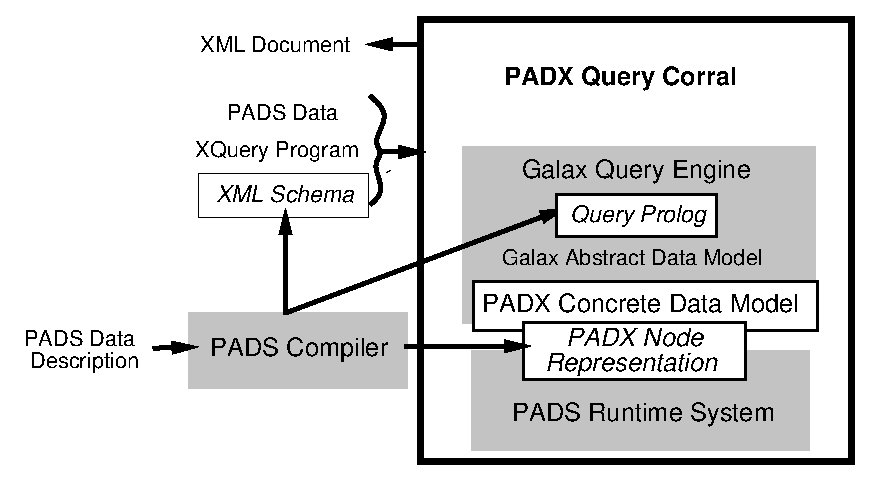
\epsfig{file=padx-arch.ps,width=0.47\textwidth}
\end{center}
\caption{\padx{} Architecture}
\label{figure:padx-arch}
\end{figure}

Put the pieces all together.  Sythesis of the two systems here. 
(Symbiotic)

\subsection{Virtual XML view of PADS data}

Embedding of PADS types in XML Schema.  One-to-one mapping from
PADS compound types to XML Schema complex types.  One-to-one mapping
from PADS base types to XML Schema simple types.  Field in compound
types are realized as local elements in XML Schema. 

All the compound types are annotated with an optional parse-descriptor
(absent if no errors occured).  Allows users to query error
structures, which may be most important data.  Other types annotated
with corresponding fields from PADS rep, e.g., arrays have a length. 

Extra level of indirection in representation of arrays---wrap each
item in an element. 

Extra level of indirection for base types: must contain the value of
the base type and an optional parse-descriptor, if an error has
occurred. 

We don't take complete advantage of XML Schema, e.g., Penum types
could be modeled by XML Schema enumeration simple types, but currently
unsupported.

Generated XML Schema.

\begin{figure*}
\begin{small}
\begin{code}
<xs:schema targetNamespace="file:sirius.p"
           xmlns="file:sirius.p"
           xmlns:xs="http://www.w3.org/2001/XMLSchema"
           xmlns:p="http://www.padsproj.org/pads.xsd">
<xs:import namespace = "http://www.padsproj.org/pads.xsd".../>
...
<xs:complexType name="\kw{order_header_t}">
 <xs:sequence>
  <xs:element name="order_num" type="p:val_Puint32"/>
  <xs:element name="att_order_num" type="p:val_Puint32"/>
  <xs:element name="ord_version" type="p:val_Puint32"/>
  <!-- More local element declarations -->
  <xs:element name="pd" type="\kw{p:PStruct_pd}" minOccurs="0"/>
 </xs:sequence>
</xs:complexType>
<!-- More complex type declarations -->
<xs:complexType name="\kw{orders_t}">
 <xs:sequence>
  <xs:element name="\kw{elt}" type="order_t" maxOccurs="unbounded"/>
  <xs:element name="\kw{length}" type="p:Puint32"/>
  <xs:element name="\kw{pd}" type="\kw{p:Parray_pd}" minOccurs="0"/>
 </xs:sequence>
</xs:complexType>
...
</xs:schema>
\end{code}
\end{small}
\caption{Fragment of XML Schema for \dibbler{} \pads{} description.}
\label{figure:dibbler-schema}
\end{figure*}

``Error-aware'' mapping from PADS type system to isomorphic XML
Schema. 
\begin{small}
\begin{code}
<xs:complexType name="\kw{val_Puint32}">
  <xs:choice>
   <xs:element name="val" type="p:Puint32"/>
   <xs:element name="pd" type="p:Pbase_pd"/>
  </xs:choice>
</xs:complexType>
<xs:complexType name="\kw{Pbase_pd}">
 <xs:sequence>
   <xs:element name="\kw{pstate}"  type="p:Pflags_t"/>
   <xs:element name="\kw{errCode}" type="p:PerrCode_t"/>
   <xs:element name="\kw{loc}"     type="p:Ploc_t"/>
 </xs:sequence>
</xs:complexType>
\end{code}
\end{small}

Example of query that uses generated schema.
\begin{small}
\begin{code}
declare namespace p = "http://www.padsproj.org/pads.xsd";
import schema default element namespace "file:sirius.p"
  schemaLocation "file:/somewhere/sirius.xsd";

$pads/p:Psource/orders/elt[events/elt[1]
  [tstamp >= xs:dateTime("2004-10-01:00:00:00") and 
   tstamp < xs:date("2004-11-01:00:00:00") ]]
\end{code}
\end{small}

\subsection{Physical Data Model}

Implementation of Galax's Abstract Tree Model.

Minimum necessary to implement Galax DM:

1. Generic implementations of the DM accessors: axis::node-test(), children(),
   attributes(), name(), etc. 

2. On PADX-side, we have a virtual handle for each node in the XML
   tree--we call that a node rep.  Node rep contains pads handle
   (maintains state for PADS parser); type-specific vtable of DM
   accessors; other stuff...

   Give example of vtable for event\_t and possibly code for
   kthChildByName. 

When to actually read from PADS data?

Options: 

1. Bulk read: Materialize entire PADS representation, populate all of the PADS
reps.  Then PADX DM lazily invoked the DM accessors over this data.
Problem: if data is big, it's all sitting in memory, even if the query
only touches a fragment of the virtual XML tree.

2. Smart read: 

Many common queries permit sequential, streamed access to underlying
XML source.  Give an example.  

Smart node rep, preserves meta-data about previously read records, but
re-uses memory for reading next item.  This rep permits multiple scans
of input (semantic problem is that DM must preserve node identity),
but slowly. 

Heuristic: records are a good level of granularity to read.   Each
smart node corresponds to one record.  When next smart node is
accessed, a little meta-data is preserved: the node rep and the
records location in the file (so we can re-read it if necessary).

3. Linear read: same as smart but does not preserve meta-data.
   Does not permit multiple scans of data source. 

Put in PADX signatures for constructing a new node and accessing
kthChild. 

\section{Performance}
\label{section:performance}

\subsection{Materialization and Loading}

Hypothesis: bulk loading should not scale for increasing document size
(limits of main memory).  Show that smart/linear does scale.

\subsection{Querying}

Give examples of queries that analyst cares about. 

Example of query that can be evaluated in single scan over data
source, but is currently not 

Database person would balk at this point!  Why aren't you just loading
this data into a real database, building indices and getting good
query performance?  B/c data is ephmeral, queries are ephmeral, but
analyst/programmer should profit from disciplined access/querying of
their data.  Don't abandon them to Perl. 

\section{Related Work}
\label{section:relatedwork}

DFDL. Contivo. 

\section{Future Work and Discussion}
\label{section:future}
Open problem: give result of XQuery and its corresponding type,
serialize result back into PADS rep.  How are the syntactic
constraints for the new values expressed?  Tool could pick default
delimiters automatically. 

Open problem: given an arbitrary PADS type, permit skipping and
reading at arbitrary positions within the data source. 

Big open problem: Given arbitrary XQuery expression, determine whether
it can be evaluated in single scan over data.  

\bibliographystyle{abbrv}
\small
\bibliography{../pldi/pads} 

\end{document}

\subsubsection{XML Generation}

\pads{} also supports converting ad hoc data into XML by providing a
canonical mapping from \pads{} descriptions into XML.  This mapping is
quite natural, as both \pads{} and XML are languages for describing
semi-structured data.  One interesting aspect of the mapping is that
we embed not just the in-memory representation of \pads{} values, but
also the parse descriptors in cases where the data was buggy.  This
choice allows users to explore the error portions of their data
sources, which can be the most interesting parts of the data.  Given a
\pads{} specification, the \pads{} compiler generates an XML Schema
describing the canonical embedding for that data source.  As an
example, the following is the portion of the generated XML Schema for
the \cd{eventSeq} type in the \dibbler{} data description.

The \pads{} compiler generates a \cd{write_xml_2io} function for each
type, an example of which is shown in \figref{figure:library}.  Given
a specification of the top level type, \pads{} can also automatically
generate a conversion program, the output of which conforms to the
generated XML Schema.

\subsection{Queries}

Our final use-scenario is querying data.  Given a data source, a
natural desire is to ask questions about the data, a desire which led
to SQL and its many variants for relational data and XQuery for XML
data~\cite{boag03XQueryDraft}.  Analysts working with ad hoc data
would also like to query their data, but the lack of tools generally
means they code their queries in an imperative fashion in languages
such as \textsc{awk}, \perl{}, or \C{}.  Indeed, the analyst working
with the \dibbler{} data took this approach.  He coded queries such as
``Select all orders starting within a certain time window," ``Count
the number of orders going through a particular state," and ``What is
the average time required to go from a particular state to another
particular state" in a mixture of \textsc{awk} and \textsc{perl}.  He
was able to get the answers to his questions, but he had to code the
queries explicitly, and the query-related code ended up embedded in
his already-brittle parsing code.

Happy with XQuery's expressiveness, we worked with the designers of
the Galax~\cite{galax} open-source implementation of XQuery to define
a data API~\cite{galaxmanual}.  This API presents the source as a tree
to Galax. With this architecture, Galax can incorporate any data
source accessible through an instance of the data API.  We then
extended the \pads{} system to produce such instances.  We were able
to define the bulk of the API generically, having to generate on a per
type basis only a handful of functions.  \figref{figure:library}
contains the key generated functions for the \cd{entry_t} type from
the \dibbler{} data.  The \cd{node_new} function creates a node in the
tree representation of the data, storing the supplied name, mask,
parse descriptor, and in-memory representation.  It makes the argument
node the parent of the newly created node.  The \cd{node_kthChild}
function takes a tree corresponding to an \cd{entry_t} node and a
child index and returns the appropriate child.  For the \cd{entry_t}
type, possible children are the header, the event sequence, or a parse
descriptor.  At the moment, it is possible to use the resulting system
to query ad hoc data sources that can be loaded entirely into memory,
and a version that allows the data to be read lazily is well underway.
How best to optimize Xqueries over ad hoc data sources is an open
research area.

PDCI_node_t *order_header_t_node_kthChild (PDCI_node_t *self,PDCI_childIndex_t idx)
{
  PDCI_node_t *result = 0;
 order_header_t *rep=(order_header_t *) (self->rep);
 order_header_t_pd *pd=(order_header_t_pd *) (self->pd);
 order_header_t_m *m=(order_header_t_m *) (self->m);
 switch(idx){
;
  case 0: result = Puint32_node_new(self,"order_num", &(m->order_num), &(pd->order_num), &(rep->order_num), "element", "order_header_t" "_node_kthChild");
 break;
  case 1: result = Puint32_node_new(self,"att_order_num", &(m->att_order_num), &(pd->att_order_num), &(rep->att_order_num), "element", "order_header_t" "_node_kthChild");
 break;
  case 2: result = Puint32_node_new(self,"ord_version", &(m->ord_version), &(pd->ord_version), &(rep->ord_version), "element", "order_header_t" "_node_kthChild");
 break;
  case 3: result = service_tn_t_node_new(self,"service_tn", &(m->service_tn), &(pd->service_tn), &(rep->service_tn), "element", "order_header_t" "_node_kthChild");
 break;
  case 4: result = billing_tn_t_node_new(self,"billing_tn", &(m->billing_tn), &(pd->billing_tn), &(rep->billing_tn), "element", "order_header_t" "_node_kthChild");
 break;
  case 5: result = nlp_service_tn_t_node_new(self,"nlp_service_tn", &(m->nlp_service_tn), &(pd->nlp_service_tn), &(rep->nlp_service_tn), "element", "order_header_t" "_node_kthChild");
 break;
  case 6: result = nlp_billing_tn_t_node_new(self,"nlp_billing_tn", &(m->nlp_billing_tn), &(pd->nlp_billing_tn), &(rep->nlp_billing_tn), "element", "order_header_t" "_node_kthChild");
 break;
  case 7: result = zip_code_t_node_new(self,"zip_code", &(m->zip_code), &(pd->zip_code), &(rep->zip_code), "element", "order_header_t" "_node_kthChild");
 break;
  case 8: result = dib_ramp_t_node_new(self,"ramp", &(m->ramp), &(pd->ramp), &(rep->ramp), "element", "order_header_t" "_node_kthChild");
 break;
  case 9: result = Pstring_node_new(self,"order_type", &(m->order_type), &(pd->order_type), &(rep->order_type), "element", "order_header_t" "_node_kthChild");
 break;
  case 10: result = Puint32_node_new(self,"order_details", &(m->order_details), &(pd->order_details), &(rep->order_details), "element", "order_header_t" "_node_kthChild");
 break;
  case 11: result = Pstring_node_new(self,"unused", &(m->unused), &(pd->unused), &(rep->unused), "element", "order_header_t" "_node_kthChild");
 break;
  case 12: result = Pstring_node_new(self,"stream", &(m->stream), &(pd->stream), &(rep->stream), "element", "order_header_t" "_node_kthChild");
 break;
  case 13: if (pd->nerr > 0) result = PDCI_structured_pd_node_new(self,"pd",pd,"ty" "_node_kthChild");
 break;
 };
  return result;
}
PDCI_node_t *order_header_t_node_kthChildNamed (PDCI_node_t *self,PDCI_childIndex_t idx,char const *name)
{
  PDCI_node_t *result = 0;
 PDCI_childIndex_t i;
 const char *fieldNames[] = {
 "order_num","att_order_num","ord_version","service_tn","billing_tn","nlp_service_tn","nlp_billing_tn","zip_code","ramp","order_type","order_details","unused","stream" , "pd",0};
 if (idx != 0) return result;
 for (i = 0;
 1;
 i++) {
 if (fieldNames[i] == 0) {
 return result;
 }
 if ((strcmp((name),(fieldNames[i])) == 0)) {
 break;
 }
 };
  return (self->vt->kth_child)(self,i);
}
